%% The first command in your LaTeX source must be the \documentclass command.
%% We use the review anonymous format for submissions - do not change this!
\documentclass[sigconf, nonacm]{acmart}
% \documentclass[sigconf, nonacm]{acmart}

%% \BibTeX command to typeset BibTeX logo in the docs
\AtBeginDocument{\providecommand\BibTeX{{Bib\TeX}}}

%% Hack to allow for comments about author contribution - not used
% \newcommand{\projectcontrib}[1]{\affiliation{\country{#1}}}

%% If you need any other LaTeX packages, add them here
\usepackage{algorithm}
\usepackage{algpseudocode}
\usepackage{verbatim}
\usepackage{svg}
\usepackage{mathtools}
\let\Bbbk\relax
\usepackage{amsmath}
\usepackage{amssymb}
\usepackage{amsfonts}

%% For managing citations, it is recommended to use bibliography files in BibTeX format.
%%
%% You can then either use BibTeX with the ACM-Reference-Format style, or BibLaTeX with the acmnumeric or acmauthoryear sytles, that include support for advanced citation of software artefact from thebiblatex-software package, also separately available on CTAN.

%% print page numbers
\settopmatter{printfolios=true} 

%% end of the preamble, start of the body of the document source.
\begin{document}

%% The "title" command has an optional parameter allowing the author to define a "short title" to be used in page headers.
\title[Robust Probabilistic Triangulation of Moving Mice]{RodenZ: Robust Probabilistic Triangulation of Moving Mice}

%% The "author" command is used to define the authors.
%% You shall sabmit the anonymised version of your paper for review, so no need to include author names here.
\author{Peter Preinesberger}
\affiliation{\institution{THWS, MAI}\city{}\country{}}
%\city{Würzburg}\country{Germany}
\author{Sandro Paval}
\affiliation{\institution{THWS, MAI}\city{}\country{}}

\author{Ivan Zelin}
\affiliation{\institution{THWS, MAI}\city{}\country{}}

% %% By default, the full list of authors will be used in the page headers. 
% %% If this is too long use "shortauthors" to define a more concise list with surnames only.
% \renewcommand{\shortauthors}{Awsomeauthor, Greatauthor, Amazingauthor}

%% The abstract is a short summary of the work to be presented in the article.
\begin{abstract}
%Although recent advances in computer vision have enabled markerless pose estimation from 2D video, most natural behaviors take place in three dimensions. 
Accurate three-dimensional tracking of movement from sequential video data is fundamental to the study of animal behavior, with a widespread approach being geometric triangulation on multi-camera sequences of 2D keypoints. These methods require accurate prior accurate camera calibration. In the context of missing calibration, the use of animal subject keypoints for joint optimization of camera parameters has been proposed. This introduces an overreliance on possibly faulty detections, and disregards the temporal structure inherent to the data. In this work, we propose leveraging tools of the Bayesian Smoothing domain to address these limitations. Our approach enables robust calibration and triangulation even in scenarios where reliable calibration sequences are unavailable, while exploiting temporal context for the inference of \emph{all} parameters, positions and calibrations, within a unified, single-stage pipeline. We demonstrate the effectiveness of our method on a dataset of freely moving mice recorded with an experimental setup of modest quality, showing highly competitive performance on the 3D pose reconstruction task.
\end{abstract}

%% Keywords: pick words that accurately describe the work being presented. Separate the keywords with commas - not used.
%\keywords{\LaTeX, template, project, MAI}
%% This command processes the author and affiliation and title information and builds the first part of the formatted document.
\maketitle

%% Add here the link to your code repository
\vspace{-0.5em}
\textbf{Code:} \url{https://github.com/thws-mai/PM25_Mice}

\section{Introduction and Related Work}
\label{sec:intro}
The analysis of animal body movements provides critical insights across a wide range of fields, especially in neurology \cite{spasojevic2015vision} and biology \cite{an1984kinematic,lu2012biomechanics}. 
%For example, it helps neurologists to monitor the progression of diseases such as Parkinson's \cite{spasojevic2015vision}, allows biologist to evaluate limb biomechanics \cite{an1984kinematic,lu2012biomechanics}, or even to quantify stress- and contaminant-induced behavioral alternations \cite{kane2004video}.
A frequently used method involves extracting two-dimensional positions of skeletal keypoints from video data of animals. CNN-based feature extractors such as DeepLabCut (DLC) \cite{mathis2018deeplabcut} and others\cite{pereira2019fast, pereira2022sleap,graving2019deepposekit,cao2019openpose,machado2015quantitative} facilitate this tracking with only few labeled frames. \par
%Although 2D detections can be sufficient to monitor certain behavior, 
However, many complex or subtle tasks require accurate 3D pose estimates, which requires lifting these 2D observations into a 3D context. Existing tools for 3D pose estimation from sequences of 2D keypoints can generally be categorized into two main approaches:. 
%Before the advent of computer vision-based methods, scientists predominantly relied on marker-based tracking approaches \cite{ZAKOTNIK200443,10.1242/jeb.042515} which require physical intervention with the test subjects. This intervention can induce stress, and alter natural movement patterns thus biasing the behavioral analysis itself \cite{garg2022markerless}. Through the progress of marker-less approaches, such as DeepLabCut (DLC) \cite{mathis2018deeplabcut}, LEAP \cite{pereira2019fast} and others \cite{pereira2022sleap,graving2019deepposekit,cao2019openpose,machado2015quantitative}, human inference with test subjects is no longer needed, given frames with annotated keypoints. These are being used to directly train a Convolutional Neural Network (CNN) to automatically detect learned joints give a new image.
\begin{itemize}
%    \item \textbf{Deep learning-based}: These methods directly infer 3D pose from images using trained neural networks, without an explicit geometric reconstruction step \cite{dunn2021geometric,zimmermann2020freipose}.
    \item \textbf{Geometric:} This approach leverages multi-view geometry, such as triangulation \cite{Nath2019}, or techniques like bundle adjustment (BA) \cite{Gnel2019}.
    %In these methods, 2D keypoints, for example obtained from a network such as DLC, are used to reconstruct 3D poses.
    \item \textbf{Probabilistic}: These approaches model pose estimation as a probabilistic inference problem, using Bayesian filtering techniques such as the Extended Kalman Filter (EKF) \cite{Joska2021}.
\end{itemize}
\begin{figure}[htbp]
  \centering
  \includesvg{example_images.svg}
  \caption{Example frames from each of the four cameras.}
  \label{example-frames} 
\end{figure}
Along with these approaches for reconstruction from 2D detections, there exists a third category of direct image-to-3D approaches based on deep learning \cite{dunn2021geometric,zimmermann2020freipose}, which have shown good results. However, these methods are heavy on computing resources, and as a result most effectively applied to short videos. However, in this work we work with videos of around 15 minutes in length, and don't consider these methods further. 

Traditionally, all of the named approaches depend on high-quality a priori camera calibration, relying on video sequences containing a checkerboard or other calibration pattern with known geometry to estimate the camera parameters \cite{zhang2002flexible}. 
%When the calibration sequences are of low quality, this initial estimation can be further refined by applying Bundle Adjustment (BA) to jointly optimize the camera parameters in a numerical framework, using 2D keypoint detections as reference points \cite{Karashchuk2021, Gnel2019}. \par
However, in many real-world scenarios, board calibrations are not realistic to obtain, either because of miniscule experiment size \cite{Gnel2019}, or because of operational issues, as is the case for our dataset. In such situations, the usage of Bundle Adjustment (BA), an optimization framework where relative camera geometry and locations of 2D observations in 3D are esimated, has been proposed to estimate camera geometry directly from the points obtained by the keypoint detector. \cite{Karashchuk2021, Gnel2019}.\par
Although this approach can work in practice, it suffers from two fundamental drawbacks:
\begin{itemize}
    \item \textbf{Overconfidence in Keypoint Detector.} Using outlier detections for BA might significantly hamper the calibration effort. This is usually addressed by only using keypoints the detector has flagged as being 'high-likelihood' \cite{Gnel2019, Karashchuk2021}, which can only serve as a mitigation, since the detector might still produce confident false positives.
    \item \textbf{Disregarding Temporal Context.} Treating the detections as individual reference points for BA loses the temporal context of the detections being points on an animal's body in time. Integrating this temporal knowledge could make for a more data-efficient approach, and lead to more robustness to the mentioned outlier detections.
\end{itemize}
%However, this calibration process depends on the availability and quality of dedicated calibration recordings. In scenarios where such data are unavailable or unusable, for example when calibration videos were not recorded or when the camera system can no longer be accessed, alternative approaches must be employed. One such method is used in DeepFly3D \cite{Gnel2019}, which uses inferred 2D joints locations as reference points for calibration. While this approach enables some calibration for recordings captured with unknown cameras, it relies on manufacturer-provided intrinsic parameters and does not constitute a full calibration procedure. Furthermore, traditional approaches such as triangulation or BA often disregard temporal context, as they are primarily constrained by the camera projection geometry. However, temporal information can be crucial for reconstructing smooth and physically consistent 3D trajectories. AniPose partially addresses this limitation through ad-hoc temporal post-processing, by applying a median filter on triangulation outputs. In contrast, the EKF used in AcinoSet\cite{Joska2021} explicitly incorporate temporal context into the reconstruction process. Nevertheless, handcrafted skeletal models for individual animals with fixed joint lengths are required in AcinoSet. This introduces an additional dependency on expert-designed anatomical models for each animal recorded, constraining the general applicability of the approach. 
Addressing these limitations, we introduce RodenZ, a robust probabilistic triangulation method for tracking freely moving mice, based on an Unscented Kalman Filter (UKF). Whereas previous probabilistic approaches only integrated temporal context into animal positions \cite{Joska2021}, RodenZ directly estimates its extrinsic and intrinsic camera parameters within the state model, integrating temoral context into the calibration process, resulting in a more robust holistic approach to the combined calibration-tracking problem.

\section{A Challenging Dataset of Mice}
\label{sec:dataset}
RodenZ was developed whilst working on a challenging dataset of mice recorded from four camera perspectives (Figure \ref{example-frames}), the raw video data having been collected by a team at the University Clinic of Würzburg. The focus of their research is the study of the impact of optogenetics on animal behaviour, a technique where neurons are stimulated using light in an attempt to elucidate their functionality\cite{Hyeon2025, Marton2016}.\par
From the raw video data, we extracted 800 Frames, uniformly distributed across camera views, by using the k-means frame clustering approach from DeepLabCut \cite{Nath2019}, producing a set of frames showing mice in a variety of poses. These frames were manually annotated with the 2D image positions of 20 keypoints, including limbs, the spine and facial keypoints.\par
% TODO: cross validation, leave one camera out, integrate this somehow ...

We applied a cross-validation-like approach in which, for each camera, a unique split of approximately 65 view-dependent frames was extracted for evaluation, while a CNN was trained on the remaining annotations. All extracted annotations originate from the same video, which was fully excluded from the training set to prevent data leakage. This strategy allows us to make the most of our limited data, as each annotation is ultimately used in the full evaluation. These annotations serve as the ground-truth 2D positions, which are then compared to the 2D projections of the 3D estimates to compute our quantitative error measure.

%We split this dataset in two, making sure that the split respects the boundary of %the videos the frames were extracted from. 
%The first set, the \emph{training set}, contains 746 frames and may be used to %train 2D keypoint detectors \cite{Nath2019}. The second \emph{evaluation set} is %to be exclusively used as a ground truth set of 2D positions, which is to be %compared with 2D projections of the 3D estimates produced by the reconstruction %methods, to form a quantitive error measure.


\par
In terms of board calibration sequences, there is a sequence of ChArUco-calibrations for three of the four cameras. Unfortunately, the bottom camera (see Figure \ref{example-frames}) was broken when the calibration sequences were recorded and was subsequently removed from the setup in order to be repaired, making it unlikely that a calibration sequence from the exact previous position of this camera will ever be recorded. In particular, this means that approaches building on checkerboard sequences are not able to use this camera.\par
Aside from the missing calibration sequence, there are other factors that make this dataset challenging. \par For one, whilst many other datasets \cite{Joska2021, Karashchuk2021} feature image resolutions of $1920\times 1080$ or higher, the footage we were provided with sits at a very modest $640\times 480$, with the actual mouse occupying a significantly smaller portion of the frame in most situations (see Figure \ref{example-frames}). Intuitively, this constitutes a significant limiting factor to reconstruction fidelity. \par
Moreover, the actual camera geometry of the setup (Figure \ref{example-frames}), is somewhat suboptimal. Unlike other experiments \cite{Gnel2019, Joska2021}, there is no camera ''behind'' the box, meaning that there are potential dead angles where key points are not visible from any camera. \par
In combination, the lacking calibration, poor camera geometry and modest resolution make this a far more challenging scenario than what is usually discussed in the literature, and will require a principled, data-efficient processing of all available knowledge over time to achieve good calibration and reconstruction. 
\section{Methodology}
\label{sec:method}
Using the training sets described in Section \ref{sec:dataset}, we trained a DLC keypoint detector \cite{Nath2019}, and used it to annotate entire sets of synchronized videos. \par
%In contrast to the established approaches, which build complex multistaged pipelines on these sequences, consisting of checkerboard calibration, refinement of calibration using bundle adjustment, geometric per-frame triangulation and finally a median filter to integrate temporal context and remove outliers \cite{Karashchuk2021, Joska2021, Gnel2019}, our approach achieves the same result using a single stage of probabilistic inference. \par 
Our method aims to compute a probability distribution of 3D mouse keypoint positions, camera locations and focal lengths at every timestep given the entire sequence of 2D keypoint detections produced by DLC for a given set of videos. We model these distributions as Gaussian and recursively calculate their parameters using a Bayesian smoothing approach \cite{Srkk2013,Thrun2008}. In the remainder of this section, we describe the modeling assumptions we made for deploying our approach. We expect the reader to be well aquainted with Bayesian Filtering \cite{Srkk2013} and fundamental computer vision topics such as the pinhole camera model and homogeneous coordinates \cite{klette2014camera}.\par
\subsection{State Model}
We need to consider keypoints and camera positions in the state model. Intuitively, if we were to consider all camera positions as unknown, the system would be overdetermined, as our measurements only contain information about relative observations of the state. For this reason, we choose one of our cameras as an ''anchor'', fixing the camera position of that camera to some sensible default. \par
The states are then vectors $\mathbf{x} \in \mathbb{R}^{D_1}$. The state contains six parameters per keypoint, seven parameters per non-anchor camera, and a field of view angle for the anchor camera, so in total $D_1 = 6K + 7(C - 1) + 1$, where $K$ is the number of keypoints and $C$ is the number of cameras. These parameters are arranged in a state vector as follows:
\begin{align*}
    \mathbf{x} = (&(\mathbf{x}'_1)^T, ..., (\mathbf{x}'_K)^T, (\dot{\mathbf{x}}'_1)^T, ...,(\dot{\mathbf{x}}'_K)^T, \gamma_1,\\
    & \Theta_2, \Phi_2, r_2, \theta_{2}^{(y)},\theta_{2}^{(x)},\theta_{2}^{(z)}, \gamma_2, ...\\
    & \Theta_C, \Phi_C, r_C,\theta_{C}^{(y)},\theta_{C}^{(x)},\theta_{C}^{(z)}, \gamma_C
    )^T
\end{align*}
Where $\mathbf{x}'_k, \dot{\mathbf{x}}'_k \in \mathbb{R}^3$ are positions and velocities of keypoint $k$, respectively. $\Theta_c, \Phi_c \in [0, 2\pi[$ and $r_c \in \mathbb{R}$ express the position of a 3D camera as altitude, azimuth and radius respectively. By default, a camera ''looks'' at the origin $\mathbf{0}\in \mathbb{R}^3$. To allow deviations in viewing direction, $\theta_{c}^{(y)},\theta_{c}^{(x)},\theta_{c}^{(z)} \in [0, 2\pi[$, forming yaw, pitch and roll angles respectively, make up for the remaining three degrees of freedom to produce a complete parametrization of camera extrinsics. $\gamma_c \in [0,\pi[$ serves to describe the camera's field of view, as the only parameter of camera intrinsics in our state. We assume measurements to be in normalized coordinates with any radial distortion already removed and aspect ratios $a_1, ..., a_C$ known, which saves us the trouble of tracking the remaining intrinsic parameters. \par
Observations $\mathbf{y} \in \mathbb{R}^{D_2}$, $D_2 = C\cdot K\cdot2$, are then simply these normalized 2D positions $\mathbf{y'}_k^{(c)}$, of every keypoint $k$, seen from every camera $c$:
\begin{align*}
    \mathbf{y} = ((\mathbf{y'}_1^{(1)})^T, ..., (\mathbf{y'}_K^{(1)})^T, ...,(\mathbf{y'}_K^{(C)})^T)^T
\end{align*}
The goal is to estimate $p(\mathbf{x}_t |\mathbf{y}_1, ...,\mathbf{y}_T) = \mathcal{N}(\mathbf{x}_t; \mathbf{m}_t, \mathbf{P}_t)$, for every frame $t \in \{1, ..., T\}$ of a video. We will discuss our specific choice of prior $\mathbf{m}_0, \mathbf{P}_0$ in Section \ref{sec:results}.
% measurement structure
\subsection{State Transition Model}
Being a simple first-order state model, we model the time-dependency between states as a linear function (adding the velocity to the position) plus a Gaussian random walk on the velocity component:
\begin{gather*}
    \mathbf{x}_{t+1} = \begin{bmatrix}
        \mathbf{I}^{(3K \times 3K)} & \Delta_t\mathbf{I}^{(3K \times 3K)} & \mathbf{0} \\
        \mathbf{0} & \mathbf{I} & \mathbf{0}\\
        \mathbf{0} &  \mathbf{0} & \mathbf{I}\\
    \end{bmatrix} \mathbf{x_t} + \begin{pmatrix}
        \mathbf{0}^{(3K)}\\
        \prescript{x}{}{}\pmb{\xi}_t\\
        \mathbf{0}^{(7(C-1) + 1)}
    \end{pmatrix}\\
    \prescript{x}{}{}\pmb{\xi}_t \sim \mathcal{N}(\mathbf{0}, \Delta_t^2\sigma_v \mathbf{I})
\end{gather*}
Where $\Delta_t$ is the time interval between frames $t$ and $t+1$, and $\sigma_v$ is the variance of the random walk on the velocity component, chosen as a hyperparameter by the user. \par
\subsection{Measurement Model}
The measurement model represents our belief of how the states $\mathbf{x}_t$ ''become'' the measurements $\mathbf{y}_t$. Algorithm \ref{alg:measurement-model} implements the deterministic part of this procedure.
\begin{algorithm}
\caption{Deterministic State Measurement $\mathbf{h}(\mathbf{x}_t)$}\label{alg:measurement-model}
\begin{algorithmic}
\Require $\mathbf{x}_t, \Theta_1, \Phi_1, r_1, \alpha_{1}^{(y)},\alpha_{1}^{(x)},\alpha_{1}^{(z)}, \gamma_1, a_1, ..., a_C$
\State $\tilde{\mathbf{y}}_t \gets \mathbf{0}$
\For{$c = 1, \dots, C$}
\State $\mathbf{V}_c \gets \mathbf{R}_z(\theta_{c}^{(z)})\cdot \mathbf{R}_x(\theta_{c}^{(x)})\cdot \mathbf{R}_y(\theta_{c}^{(y)})\cdot \mathbf{T}_z(-r_c)\cdot\mathbf{R}_x(\Theta_c)\cdot \mathbf{R}_y(\Phi_c)$ 
\State $f_c \gets {tan(\frac{1}{2}\gamma_c)}^{-1}$
\State $\mathbf{P}_c \gets \begin{bmatrix}
    \frac{f_c}{a_c} & 0 &0 & 0 \\
    0 & f_c & 0 & 0 \\
    0 & 0 & -1 & 0
\end{bmatrix}$
\For{$k = 1, \dots, K$}
\State $\mathbf{p} \gets \mathbf{P}_c\mathbf{V_c}\begin{pmatrix}
    \mathbf{x'}_k \\ 1
\end{pmatrix}$
\State ${\tilde{\mathbf{y'}}}_k^{(c)} \gets \frac{1}{\mathbf{p}_3}(\mathbf{p}_1\,\, \mathbf{p}_2)^T$
\EndFor
\EndFor
\State $\mathbf{h}(\mathbf{x}_t) \gets \tilde{\mathbf{y}}_t $
\end{algorithmic}
\end{algorithm}
In words, the algorithm first forms view matrices $\mathbf{V}_c$ and projection matrices $\mathbf{P}_c$ for every camera. The view matrices are formed by multiplying a series of homogenous rotation matrices $\mathbf{R}_{[\,\cdot\,]}(\cdot)$, where the subscript denotes axis of rotation, and homogenous translation matrices $\mathbf{T}_{[\,\cdot\,]}(\cdot)$, where the subscript denotes the axis of translation. The projection matrices are formed from the field of view parameters $\gamma_c$ and aspect ratios $a_c$. Finally, we simply project each keypoint into each camera using these matrices. \par
To account for noise in the measurement process, we consider our measurement model to be this deterministic projection plus some additive Gaussian noise in image space:
\begin{gather*}
    \mathbf{y}_t = \mathbf{h}(\mathbf{x}_t) + \prescript{y}{}{}\pmb\xi_t \\
    \prescript{y}{}{}\pmb\xi_t \sim \mathcal{N}(\mathbf{0}, diag(\prescript{y}{}{}\pmb\sigma_t))
\end{gather*}
Where the covariances we consider for our measurements $\prescript{y}{}{}\pmb\sigma_t$ depend on how much we ''trust'' our keypoint detector at time $t$. In practice, when the keypoint detector reports a high uncertainty for a given keypoint $k$ in a given camera $c$, we will increase the respective variance entries in $\prescript{y}{}{}\pmb\sigma_t$, whereas we will set some lower value for those keypoints where the detector is ''sure'' about it's prediction. \par
We then obtain the parameters $\mathbf{m}_t, \mathbf{P}_t$ for the distributions $p(\mathbf{x}_t |\mathbf{y}_{1:T})$ $= \mathcal{N}(\mathbf{x}_t; \mathbf{m}_t, \mathbf{P}_t)$ by running a forward pass of Gaussian filtering (UKF) using these three models, and a backward pass of RTS-Smoothing \cite{Srkk2013}.\par
Our methodology is implemented as a collection of command-line tools, each guiding the user through one step of the pipeline (inference of 2D keypoints, removal of radial distortion, and finally reconstruction), and may be found using the GitHub link in the abstract.

\section{Results}
\label{sec:results}
We compared RodenZ to the predominant BA-Triangulation methodolgy, calculating the reprojection error of inferred 3D sequences to 2D labels from the \emph{evaluation set} of Section \ref{sec:dataset} as a quantitative score. \par
For both methodologies, we first trained a DLC keypoint detector using the \emph{training set} described in Section \ref{sec:dataset}, and inferred 2D keypoint positions for the videos from which we extracted the labeled frames of the \emph{evaluation set}. We then used RodenZ and AniPose to reconstruct 3D trajectories and camera poses for these videos. \par 
For RodenZ, we had to decide on a prior distribution of 3D positions and camera poses, measurement variances $\prescript{y}{}{}\pmb\sigma_t$ and a velocity variance $\sigma_v$. \par
As the real mouse box is a cube of roughly $30cm$ side length, we chose the imagined origin of our frame of reference to be the center of the cube floor, and used $cm$ as the units to describe the distance-related hyperparameters. We then chose camera positions of the format described in Section \ref{sec:method}, by aligning a rendered virtual rendition of the box with the frames that can be seen in Figure \ref{example-frames}, using the camera parameters obtained this way for the fixed anchor camera and prior means of the varying cameras respectively. For the mean prior mouse position, we assumed Gaussians centered at the floor of the box, with some prior variance covering the volume of the box generously. \par
For the measurement variances $\prescript{y}{}{}\pmb\sigma_t$, we assumed variance values based on thresholds set on the keypoint likelihood reported by the DLC predictor \cite{Nath2019}. We used likelihood thresholds of $0.6$ and $0.8$. We observed empirically the two-dimensional variance of the difference of the training set annotations and the DLC outputs at these likelihood thresholds, and used these to set the values in $\prescript{y}{}{}\pmb\sigma_t$. \par
Choosing $\sigma_v$ proved to be difficult to do in a principled way, as expert knowledge on ''mouse agility'' was not available at implementation time. In practice, we reconstructed some 3D trajectories (that were not part of the dataset), and simply observed the 3D reconstructions obtained for different values. We then chose the actual quantity by human judgment, based on if details of movement were visually preserved without observing the 'jumpiness' indicative of the RTS explaining outliers with high velocity noise. We settled on a variance of $\sigma_v = 5$ for our setup. \par

\subsection{Evaluation}
To facilitate a quantitative comparison, we picked out the reconstructed 3D positions at the timesteps where we have manual 2D labels in the evaluation set, and reprojected those 3D points to the image plane. The difference in reprojected 3D position and 2D ground truth labels was then used to estimate the quality of the 3D point. We used the distribution of 2D reconstruction error as our main method for comparison, keeping in line with the established literature \cite{Karashchuk2021}. \par
For the BA-Triangulation methodology, we adopted the AniPose\cite{Karashchuk2021} package. As we have no calibration sequences for the bottom camera, the classical approach of calibrating with boards using bundle adjustment (BA) and then triangulating, which we will call the \emph{BA-Board} approach, is not deployable to the full setup in our case. Nonetheless, we ran this approach on the remaining three cameras, comparing it to a rendition of RodenZ artificially limited to the same three cameras. We also used a feature of AniPose, where the initial board calibrations can be further refined using bundle adjustment of detected keypoints \cite{Karashchuk2021}, which we refer to as \emph{Animal-BA}. \par
For the full setup of four cameras, we evaluated if extracting the camera calibrations learned by RodenZ and using them as starting parameters for a four-camera version of Animal-BA could perhaps lead to better reconstruction performance. This implements the established calibration from keypoints procedure described in Section \ref{sec:intro}, which requires plausible starting parameters \cite{Gnel2019}. In this way, we achieve a comparison of how good the calibration is on the four-camera setup: If BA found better calibrations, it would manifest as a decrease in reprojection error.\par
The distribution of error of each approach on the limited three-camera version of the dataset can be seen in Figure \ref{fig:three-cam-hist}. We can see that in this three camera version of the dataset, the distribution of reprojection error of RodenZ and Animal-BA match almost exactly, both being vastly superior to the board calibrations alone. RodenZ does not exceed the classical performance on this task, it is nonetheless worthwhile to note that we can reproduce a very good result on this task without relying on initial board calibrations. 
\begin{figure}
    \centering
    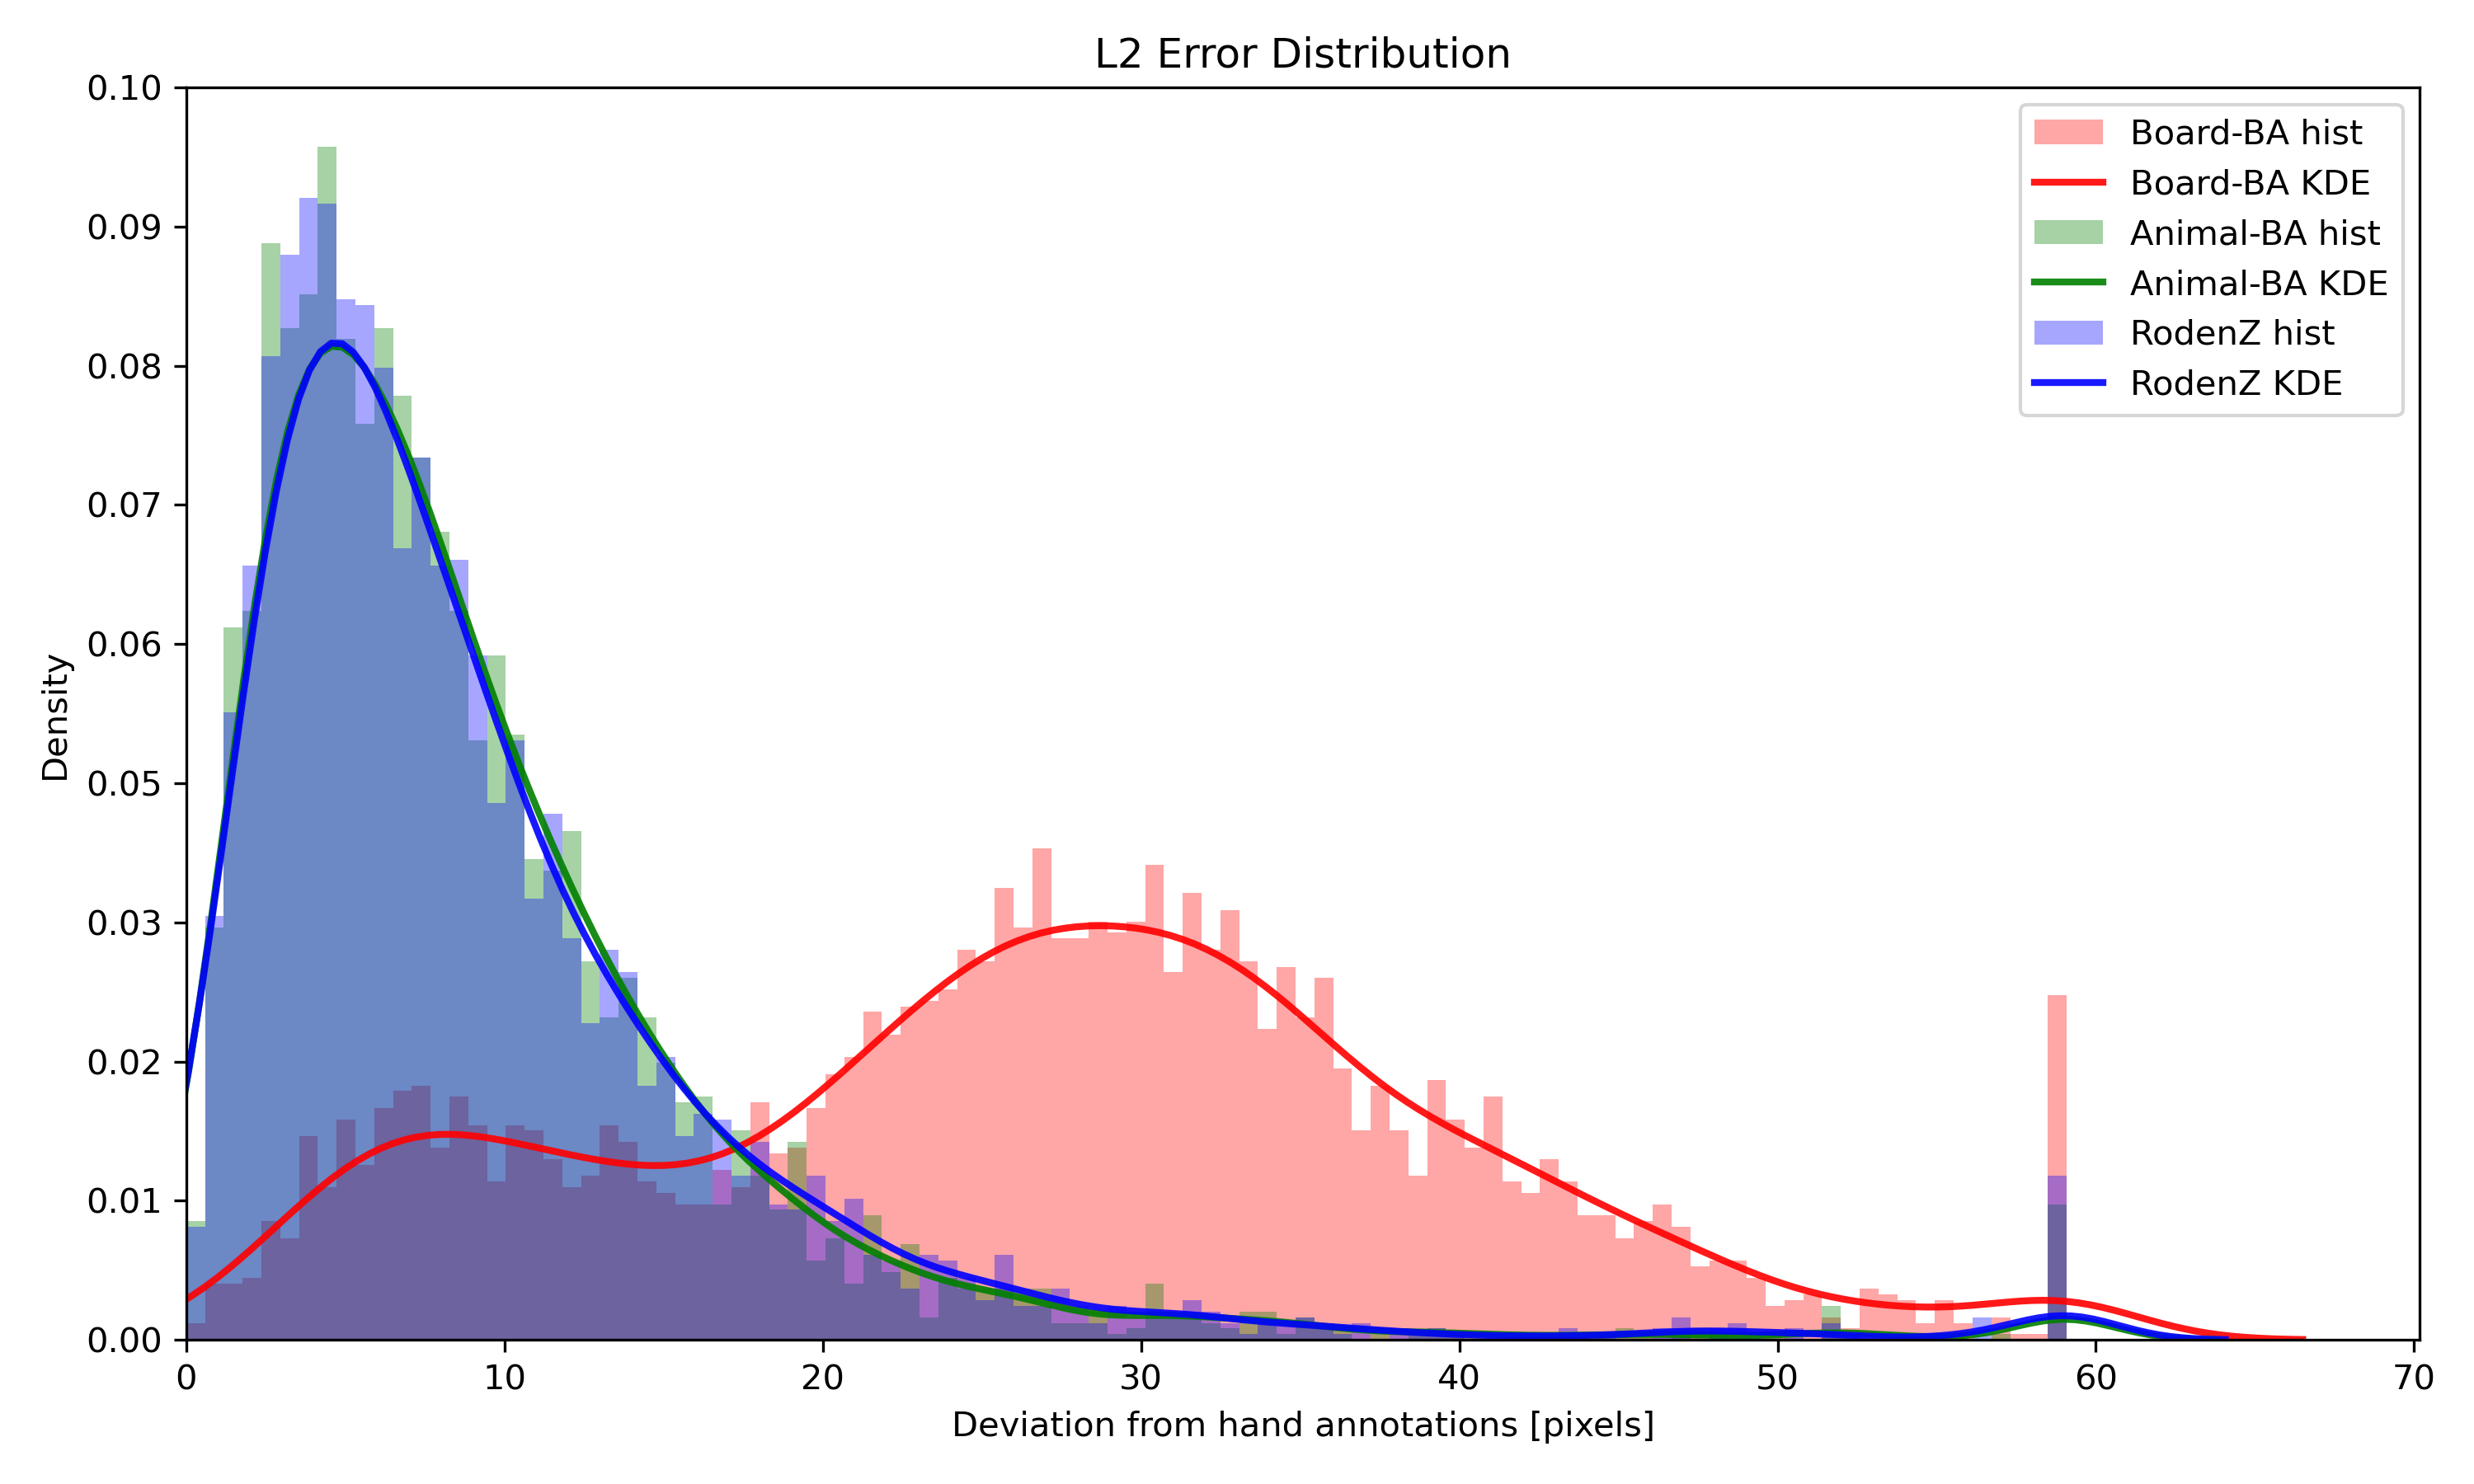
\includegraphics[width=1\linewidth]{images/plots/three_cam_hist_l2.png}
    \caption{Error distribution for the three-camera task.}
    \label{fig:three-cam-hist}
\end{figure}
\par

Of the approaches discussed here, only RodenZ is natively deployable to the four-camera setup. Observing the distribution of reconstruction errors for the full setup (Figure \ref{fig:four-cam-hist}), we see RodenZ taking the lead over the Animal-BA version that was initialized with calibrations extracted from the RodenZ run. Animal-BA noticably degrades the reconstruction error, even though it starts from initial calibrations of very high quality, as indiciated by the good RodenZ performance. A potential reason for the degrading of calibrations through Animal-BA in this case might lie with the camera perspective of the added camera being unlike the others. As the previous three perspectives were all taken from the side, there was less training data in the training set for the 'bottom' perspective, possibly leading to worse keypoint detector performance in that camera. This may have enabled confident false positive keypoints, leading the BA optimization away from the good initial calibrations. \par
\begin{figure}
    \centering
    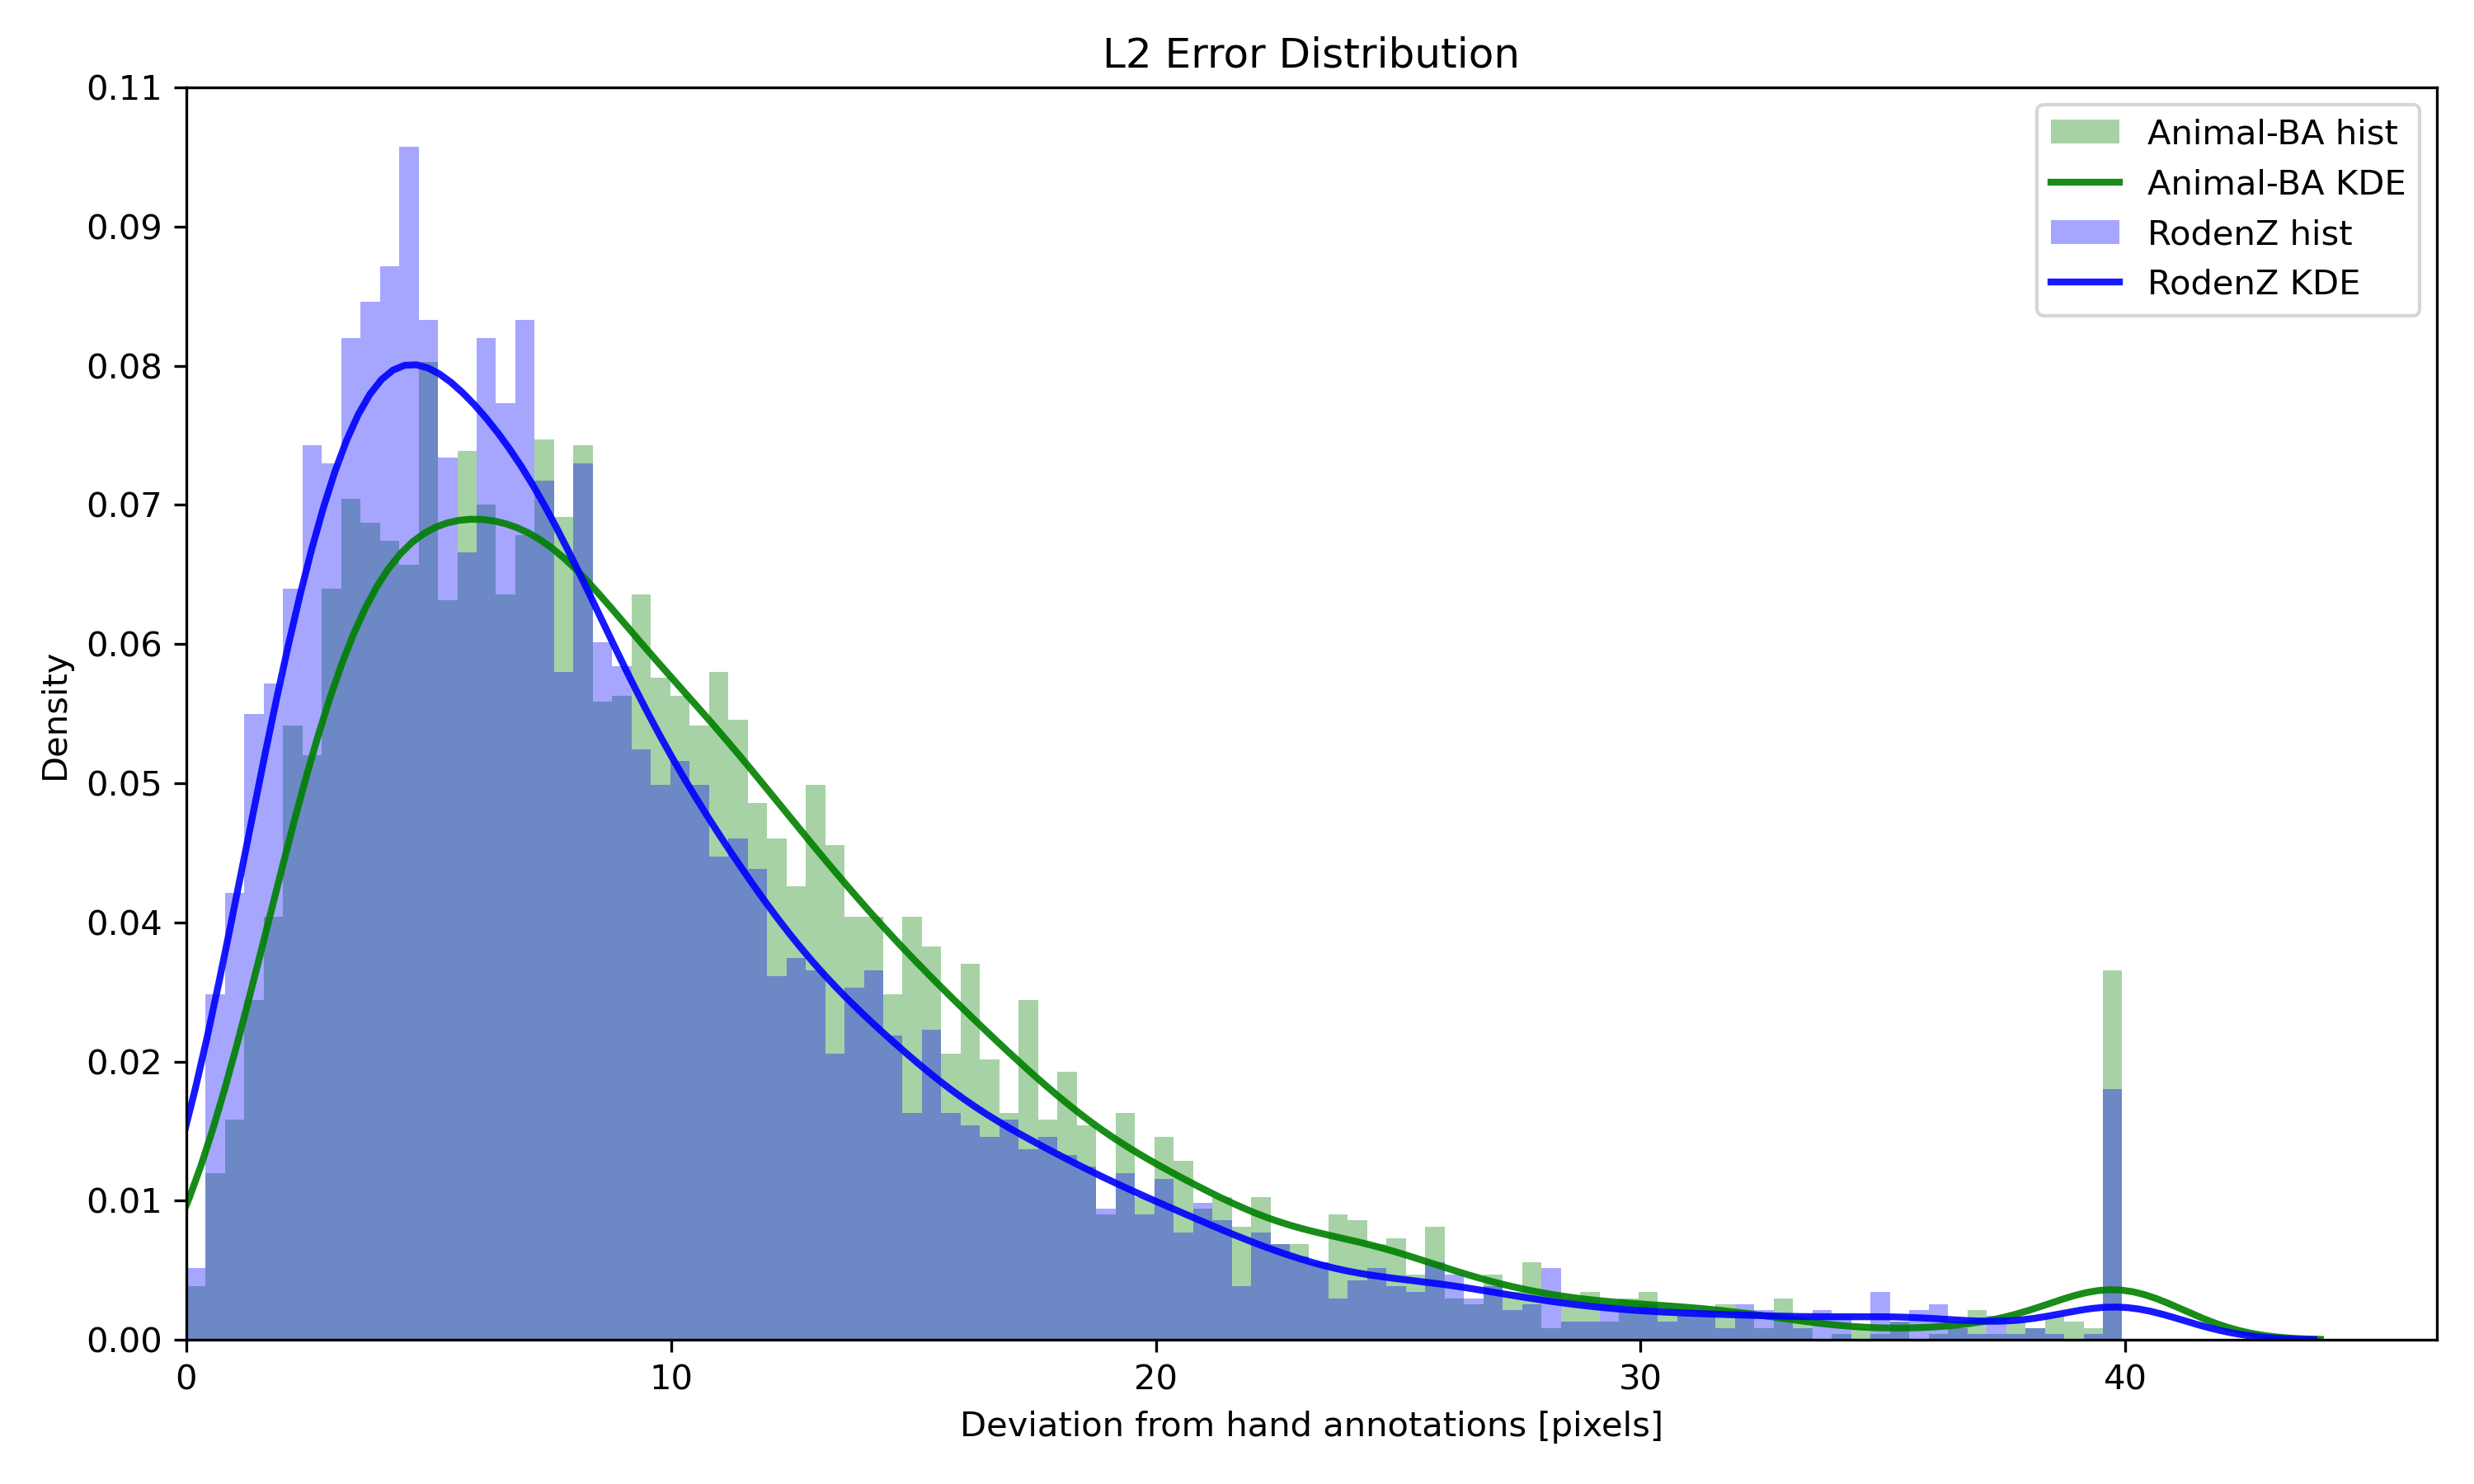
\includegraphics[width=1\linewidth]{images/plots/four_cam_hist_l2.png}
    \caption{Error distribution for the full task.}
    \label{fig:four-cam-hist}
\end{figure}
%Also, as can be observed in Table \ref{tbl:cam4}, the four camera setup sees our approach taking the lead over a version of Animal-BA initialized with the RodenZ calibrations. As both approaches now work on an even playing field of camera calibrations, the lead may be explained by RodenZ' more principled approach of leveraging temporal context in triangulation, whereas AniPose uses the ad-hoc approach of median filtering. \par

%\begin{table}[htbp]
%\begin{centering}
%\begin{tabular}{|c||c c c |} 
% \hline
% 3 Cams & Board-BA & Animal-BA & RodenZ \\[0.5ex] 
% \hline\hline
% L1   &    33.86  &     \textbf{11.88}  & 12.40   \\ 
% \hline
% L2   &    27.06 &     \textbf{9.36}& 9.82 \\
% \hline
% RMSE &    30.51 &     \textbf{13.49} & 14.13 \\
% \hline
%\end{tabular}
%\end{centering}
%\caption{Reprojection error for the three-camera subtask.}
%\label{tbl:cam3}
%\end{table}

%\begin{table}[htbp]
%\begin{centering}
%\begin{tabular}{|c||c c|} 
% \hline
%   4 Cams    & Animal-BA & RodenZ  \\ [0.5ex] 
% \hline\hline
% L1   & 13.71      & \textbf{12.98}  \\ 
% \hline
% L2   & 10.79    & \textbf{10.16}   \\
% \hline
% RMSE  & 13.83     & \textbf{13.46} \\
% \hline
%\end{tabular}
%\end{centering}
%\caption{Reprojection error for the full dataset.}
%\label{tbl:cam4}
%\end{table}

Overall, the quantitive experiments display some nuanced results. Whilst we did not manage to beat the established methodology of Animal-BA for the three-camera subtask, underscoring the effectiveness of the established method, we observed superior performance in reprojection when setting out from  calibrations supplied by our approach for the four-camera task. We attribute this to our approach being more robust to outliers that result from overconfident keypoint detections in an unusual camera perspective.\par


\section{Limitations}
We only measured the reprojection error for a quantitive evaluation of our approach, which summarizes over many aspects of a complex reconstruction system. One important quantity that we did not have the opportunity yet to evaluate is fitness for medical or biological processing down the line. A potential threat to the validity of our approach is that important aspects of animal behavior that only manifest in very fine movements are simply not visible in the smoothing output, because of the increased filtering of outliers. \par
Should it be the case that the 3D reconstructions are unfit for downstream processing, one could still use RodenZ as a standalone calibration procedure, and use the parameters obtained this way in a triangulation scheme that keeps these important details better preserved. \par
% oversmoothing removes relevant details?
\section{Conclusion and Future Work}
% todo: limitations (smoothing removes medically relevant stuff?)
We demonstrated a robust probabilistic triangulation and calibration approach on a challenging task of skeletal keypoint reconstruction. By designing a unified pipeline, we were even able to integrate information from non-calibrated cameras. Furthermore, our approach matches SotA on the calibratable subset of our task, and outperforms competing methods on the full task, even when competing approaches are allowed to exploit the calibration parameters obtained from our approach. \par
In the future, our approach could be refined by leveraging recent research on improved keypoint detectors \cite{Biderman2024}, or be extended to include anatomical constraints in the state transition model, such as joint lengths \cite{Joska2021}. Also, one could strive to include radial camera distortion parameters in the state estimation, if these are not easy to obtain a priori for a given scenario.

\bibliographystyle{ACM-Reference-Format}
\bibliography{references}

%% We use anonymised submissions for review, so do not include acknowledgements here.
% \section*{Acknowledgements}
% We thank Prof. Dr. Expert Inthefield for supervising our project and PhDStudent VeryHelpful for his valuable advice on many things we would otherwise never figure out.

%% If your work needs an appendix, this is the place to put it.
%\appendix

%\section{Appendices}\label{sec:Appendices}
%\subsection{Plots}





%\subsection{Old Intro stuff (so I dont forget it)}
%Analyzing  behavioral patterns based on body movements of test subjects is possible for human observers, however, these approaches are limited by human capacity. Some movements may be too fast or small too subtle to be actively detected, and observers are prone to fatigue \cite{ANDERSON201418}. Moreover, such tasks are often labor intensive and time-consuming, increasing the risks of human-induced errors even more. Computational methods enable us to not only analyze these patterns at a bigger scale but also at resolutions outside of human capacity \cite{dell2014automated}.
\end{document}
%% End of file `thws-mai-pm-template.tex'
